%!TEX root = ../Thesis.tex
\lstset {language=C++}
\lhead{\emph{Visual Scripting}}

\chapter{Visual Scripting}
\label{ch:visualscripting}
In dit hoofdstuk word een introductie gegeven van een visuele programmeer taal. Daarna word er als voorbeeld een vergelijking gemaakt tussen C++ en een visuele taal.

\gls{vs} maakt het mogelijk om logica op een visuele manier in plaats van tekstueel te schrijven. Er is minder kennis van de onderliggende werking van computer systemen nodig dan voor tekstueel programmeren [?]. Hierdoor kan er zonder kennis van computers en hun werking al snel mee gewerkt worden door niet programmeurs. 

\begin{figure}[!ht]
  \centering
    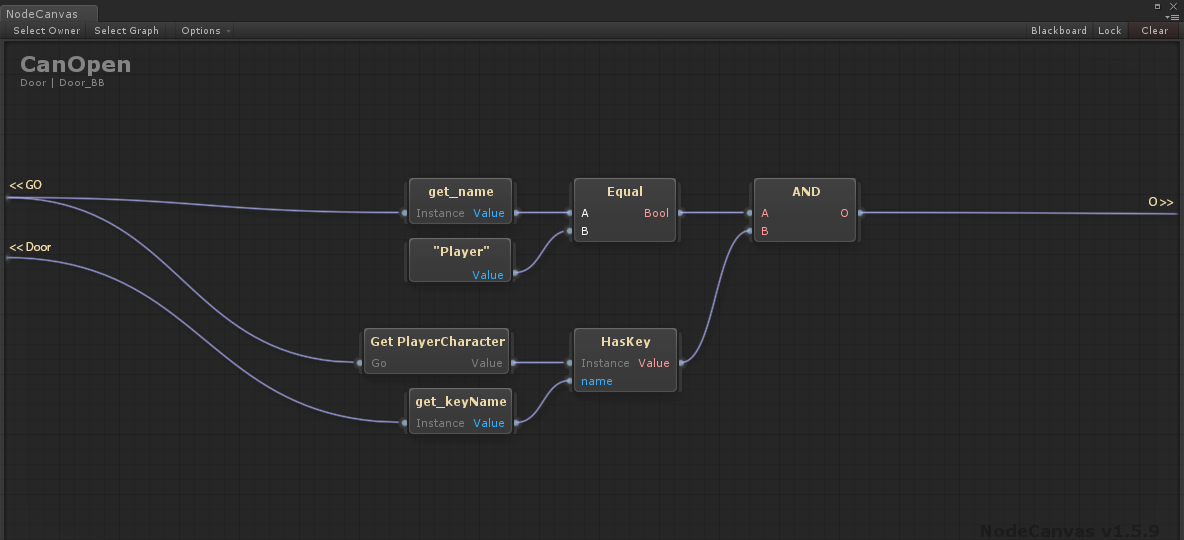
\includegraphics[width=\linewidth,height=\textheight,keepaspectratio]{VisualScriptingExample}
    \caption{Voorbeeld van een visuele script taal.}
\end{figure}

Daarnaast word de mogelijkheden van de visuele programmeer taal ook vaak gelimiteerd om het de gebruiker makkelijker te maken en het programma te beschermen van de gebruiker. Meestal als de limitaties van \gls{vs} een probleem worden had de logica beter in een tekstuele taal geschreven kunnen worden.

\section{Use Case's}
Door de jaren heen zijn er voor verschillende doeleinden visuele programmeer talen gemaakt. 
Een aantal voorbeelden zijn

\begin{itemize}  
\item Data flow in applicaties 
\item State flow voor onder andere animaties 
\item Geluids effecten programmeren
\item Gameplay Logica 
\item Programeren leren aan beginners 
\end{itemize}

In deze scriptie word er gefocust op het gebruik van \gls{vr} voor gameplay logica.

\section{Blueprints}
Blueprints is het visuele scripting systeem van \gls{ue4} en wat deze scriptie mogelijk maakt. De beschrijving van Unreal zelf is als volgt:

“Blueprints are special assets that provide an intuitive, node-based interface that can be used to create new types of Actors and script level events; giving designers and gameplay programmers the tools to quickly create and iterate gameplay from within Unreal Editor without ever needing to write a line of code.”

Blueprints ziet er als volgt uit:

\begin{figure}[H]
  \centering
    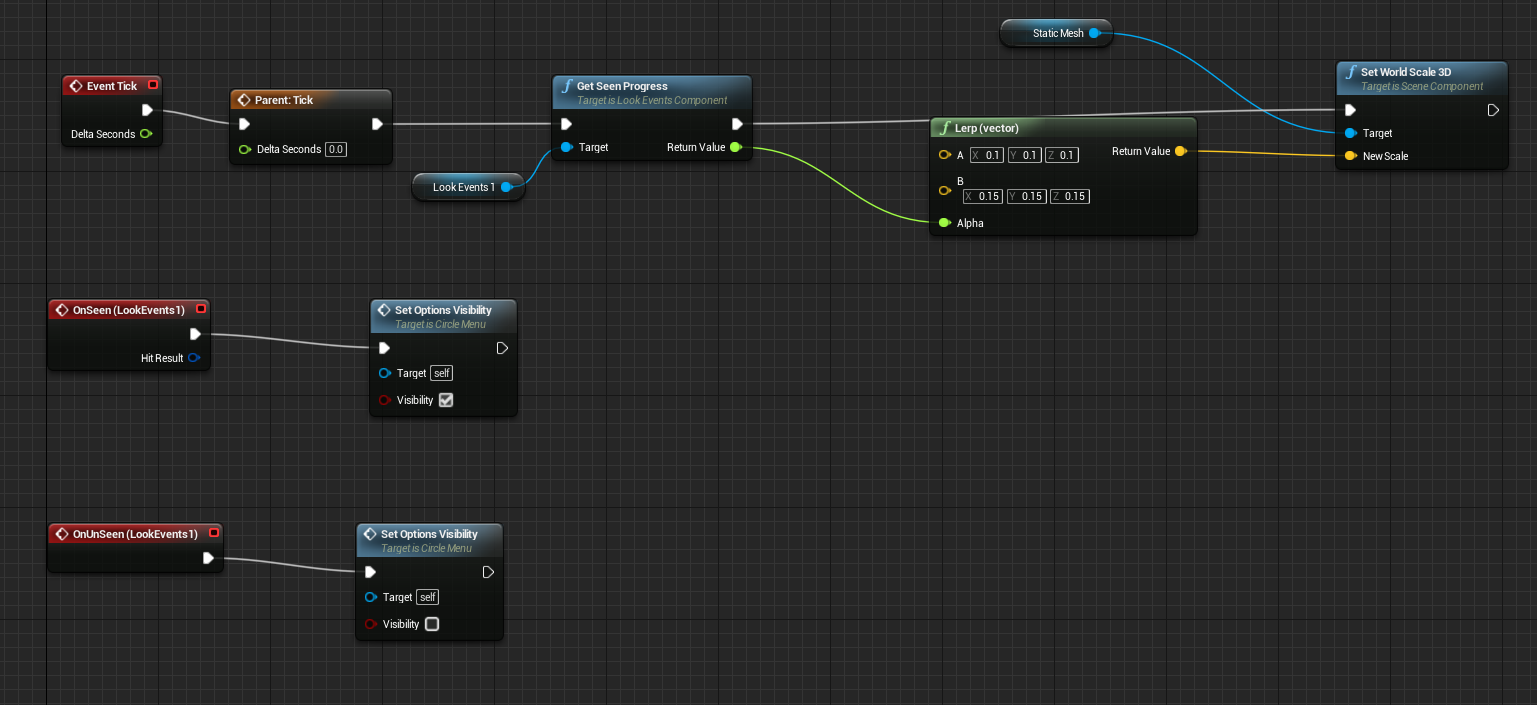
\includegraphics[width=\linewidth,height=\textheight,keepaspectratio]{BluePrintSeenExample}
    \caption{Voorbeeld van een Blueprint.}
\end{figure}

Een hele kort samenvatting zou zijn dat de rode nodes Events zijn en dus aangeven wanneer iets gebeurd, de witte lijnen bepalen de volgorde waarin de nodes worden uitgevoerd, de blauwe nodes zijn functies en de rest zijn variabelen of pure transformatie van data.

\section{Gameplay Logica}
Het programmeren van gameplay in een spel bestaat voor een groot gedeelte uit de vragen “Wanneer moet iets gebeuren”, “Wat moet er gebeuren” en “Hoe moet dit gebeuren”.
De vragen “Waarom moet iets gebeuren” en “Waar moet dit gebeuren” komen het meeste voor in de gameplay logica van een spel, vaak hebben deze vragen ook een makkelijk antwoord. Helaas zijn deze vragen lastig om te beantwoorden in tekstuele code.

\subsection{Het afvuren van een projectiel}
Een voorbeeld van deze drie vragen in code is als volgt, voor het voorbeeld laten wij de logica zien van het schieten van een projectiel in c++ gebaseerd op het standaard voorbeeld van een speler uit de \gls{ue4}.

\subsubsection{Tekstuele Implementatie}
In een c++ header bestand registreren wij de volgende functie in onze speler classe.
\begin{lstlisting}[caption=Registratie van de OnFire functie]
void OnFire();
\end{lstlisting}
Dan tijdens het opzetten van de input voor ons karakter laten we weten wanneer we een projectiel willen schieten.

\begin{lstlisting}[caption=Koppellen van de Fire actie aan de OndFire functie]
if( EnableTouchscreenMovement(InputComponent) == false )
{
	InputComponent->BindAction(
		"Fire", 
		IE_Pressed, 
		this, 
		&Adpi_unreal_colosseumCharacter::OnFire
	);
}
\end{lstlisting}
Maar omdat de “fire” actie niet werkt op een touch interface moeten we de onfire zelf afvuren als iemand het scherm aanraakt (De logica achter het registeren van touch events word niet getoond maar is wel aanwezig in de speler klasse).

\begin{lstlisting}[caption=Aanroepen van de OnFire functie tijdens het EndTouch event]
void Adpi_unreal_colosseumCharacter::EndTouch(const ETouchIndex::Type FingerIndex, const FVector Location)
{
	if (TouchItem.bIsPressed == false)
	{
		return;
	}
	if( ( FingerIndex == TouchItem.FingerIndex ) && (TouchItem.bMoved == false) )
	{
		OnFire();
	}
	TouchItem.bIsPressed = false;
}
\end{lstlisting}
Vervolgens definiëren we OnFire als volgt

\begin{lstlisting}[caption=Implementatie van de OnFire functie]
void Adpi_unreal_colosseumCharacter::OnFire()
{ 
	// try and fire a projectile
	if (ProjectileClass != NULL)
	{
		const FRotator SpawnRotation = GetControlRotation();
		// MuzzleOffset is in camera space, so transform it to world space before offsetting from the character location to find the final muzzle position
		const FVector SpawnLocation = GetActorLocation() + SpawnRotation.RotateVector(GunOffset);

		UWorld* const World = GetWorld();
		if (World != NULL)
		{
			// spawn the projectile at the muzzle
			World->SpawnActor<Adpi_unreal_colosseumProjectile>(ProjectileClass, SpawnLocation, SpawnRotation);
		}
	}

	// try and play the sound and fire animtation if specified
	...

}
\end{lstlisting}
Om de logica te implementeren voor het vuren vuren van de kogel hebben wij nu op vier verschillende plekken de logica moeten verspreiden, hiervan zit de implementatie verspreid in een bestand van 218 regels \ref{appendix:dpi_unreal_colosseumCharacter}.

\subsubsection{Visuele Implementatie}
De “Hoe moet dit gebeuren” is een complexe vraag die prima beantwoord word in code. Vooral omdat er verschillende logica achter elkaar plaatsvind, geluid afspelen / animatie starten, en een aantal wiskundige berekeningen. 

Maar de “Wanneer” vraag is makkelijk te beantwoorden. Namelijk als de fire actie uitgevoerd word of als er op het scherm gedrukt word. De logica in blueprints ziet er als volgt uit (in de event graph van een playerCharacter).

\begin{figure}[!ht]
  \centering
    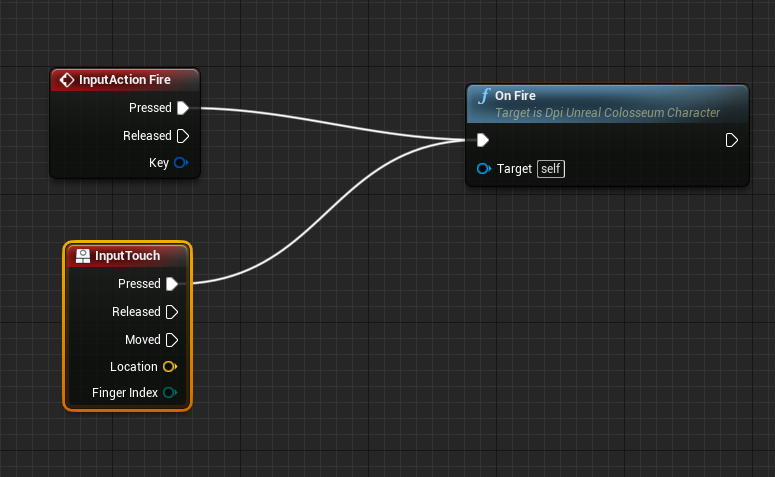
\includegraphics[width=\linewidth,height=\textheight,keepaspectratio]{OnFireBlueprintCall}
    \caption{Afvuren van een projectiel in Blueprints.}
\end{figure}

In tegenstelling tot de c++ code is de logica van de “Wanneer” vraag dit maal niet verspreid en is het in een oog opslag duidelijk wat er voor zorgt dat er een projectiel geschoten word.